% Created 2017-03-27 seg 18:05
% Intended LaTeX compiler: pdflatex
\documentclass{report}
               \pagestyle{fancy}
\usepackage[latin1]{inputenc}
\usepackage[T1]{fontenc}
\usepackage{graphicx}
\usepackage{grffile}
\usepackage{longtable}
\usepackage{wrapfig}
\usepackage{rotating}
\usepackage[normalem]{ulem}
\usepackage{amsmath}
\usepackage{textcomp}
\usepackage{amssymb}
\usepackage{capt-of}
\usepackage{hyperref}
\usepackage{paralist}
\usepackage{tcolorbox}
\usepackage[table]{xcolor}
\usepackage{lipsum}
\usepackage{caption}
\usepackage{tabu}
\usepackage[subpreambles=true]{standalone}
\usepackage{import}
\usepackage{setspace}
\usepackage{graphics}
\usepackage[linktocpage=true]{hyperref}
\usepackage{tocloft}
\usepackage{minitoc}
\usepackage[portuguese, english]{babel}
\usepackage[utf8]{inputenc}
\date{}
\title{}
\hypersetup{
 pdfauthor={},
 pdftitle={},
 pdfkeywords={},
 pdfsubject={},
 pdfcreator={Emacs 25.1.90.1 (Org mode 9.0.5)},
 pdflang={English}}
\begin{document}

\thispagestyle{firststyle}
\IssueTitle{Market Discipline or a Fallout}
\NewsAuthor{Joao Mauricio Rosal, \small\it Chief Economist, PhD}
\NewsEmail{joao.rosal@bgcpartners.com}
\JournalIssue

    \begin{tcolorbox}[colbak=red!5!white, colframe=red!0!white]
      \NewsItem{Market Discipline or a Fallout?}
      \begin{compactitem}
      \item \textit{We understand the balance of risks have tilted to the downside as odds of a muddling through type of social security reform have increased.}
      \item \textit{This implies a two-fold path going foward: a) market discipline forces the political class to embrace a meaningful reform,
                    or b) political forebearnace regnin in entailing a negative re-pricing for the longer term.}
      \itme \textit{The odds of a volatility free path towards a significant reform seems very low at moment.}
      \end{compactitem}
    \end{tcolorbox}
\vspace{-0.5cm}


\section{The Two-fold paths}
\label{sec:org5e807ff}
\begin{compactitem}[$\diamond$]
\item \textbf{Balance of risks have tilted}. The latest flow of news have
confirmed the difficulties of Mr. Temer to approve his social
security reform as is. While some type of compromising has been
expected from the outset, we believe the latest announcement to
leave State civil servants out of the reform has opened a Pandora
box, making difficult to predict what is going to come out of it.

\item \textbf{The Genie out of the box}. Simply put, once one makes a
compromising to a specific class entreched interests, the incentives
are such that other organized classes should soon start to lobby for
the same type of favoritism. In addition, there is also the interest
of less organized citizens, such as those living off social
benefits, who are held pretty close to the heart of politicians in
Brasilia. Hence, once we sum all this up, the budget of acceptable
concessions may well fall shot of all mounting pressures arising
either within politicians class or from specific sectors of the
society.

\item \textbf{Any counteracting pressure?} In light of the fore mentioned, the
easy path towards a reform that comprises a) an increases the
minimum retirement age to 65 for both genders; b) the end retirement
linked to the numbe of years contributing to the system; and c)
encompasses rural, urban, private and public workers alike, looks
very slim. In nutshell, all these theme seems far too much to fit in
the budget of the demands which currently floating around. In fact,
if we are to witness any satisfactory compromising, counteracting
forces aganist these pressure  are of paramount importance, and in this respect the market
looks like the main candidate that may step up and take up this
role.
\end{compactitem}

\begin{figure}[h]\centering
\subfloat[#]{\label{fig:spreads}
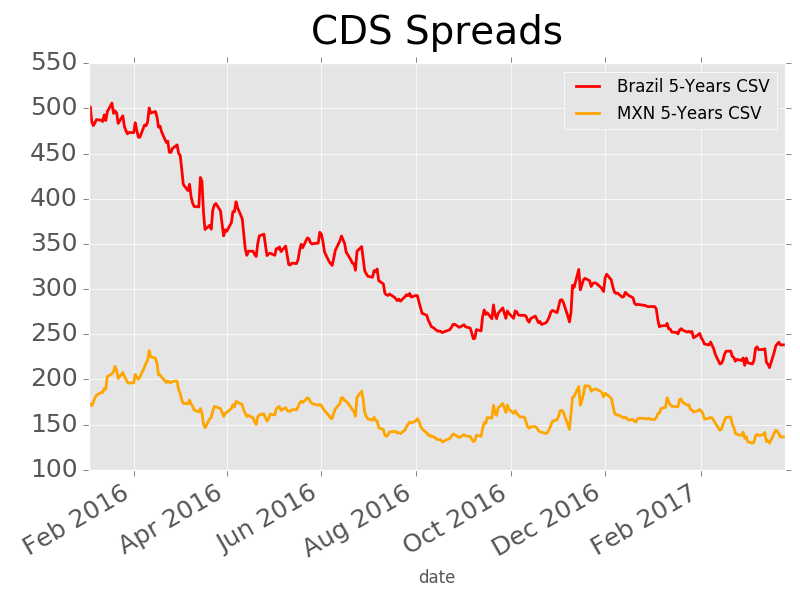
\includegraphics[width=7.5cm]{./images/csv.png}
}
\subfloat[#]{\label{fig:vol}
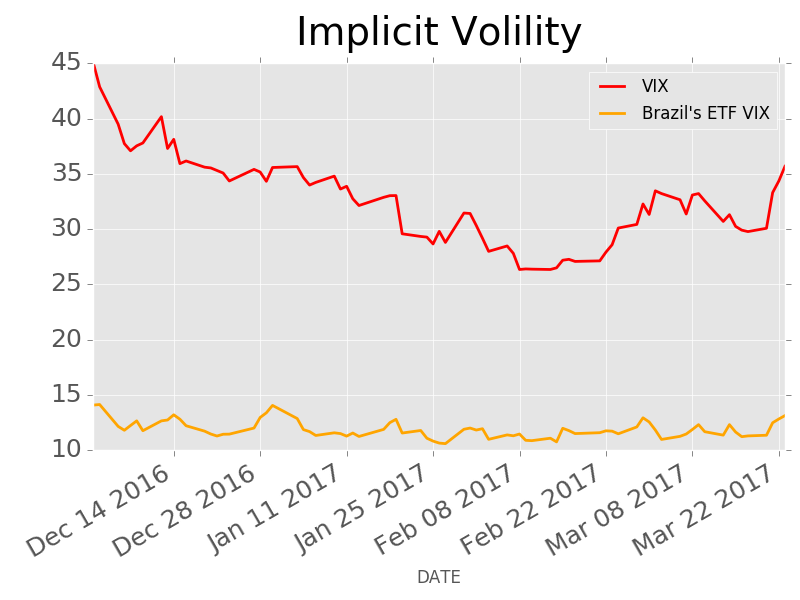
\includegraphics[width=7.5cm]{./images/vix.png}
}
\end{figure}

\begin{itemize}
\item \textbf{A two-fold path}. As in \ref{fig:spreads}, Brazilian sovereign
spreads have been standing about 90bps above Mexico's year-to-date,
a country holding a sovereign credit rating about 4 notches above
Brazil's. No doubt, it entails a rather benign vision towards the
country's outlook, in particular, with respect to the country social
security system.  Hence, should this perception changes
significantly, there is plenty of room for things to turn sour. In
fact, the recent moves concerning the social security reform have
not been shrugged off by the market, and the volatility of Brazilian
assets have clearly take off way from the US's benchmark (\ref{fig:vol}).

Hence, the question: will the political class remain oblivious to
that and follow their own agenda, or will the kneel to market
pressures? We thinks latter of the most likely candidate, but with
2018 general elections take over their agenda, one should not
dismiss the former altogether.

\item \textbf{A new Round of Reforms}. Be all that as it may, what is become
clear is that Mr. Temer's reform won't be any silver bullet to fix
social security structural under-funding, as just like the reforms
of his predecessors. In fact, with State and municipalities left out
and plus other concessions that we are yet to see, the budget of
changes for 2019 and beyond is growing, and if history is repeat
itself, they should only be ticked off with pressure coming
market.
\end{itemize}



\newpage



\section{Forecasts}
\label{sec:orgefb4c8b}


\rowcolors{2}{grey!15}{white}
\begin{center}
\begin{tabular}{lrrr}
\hline
\textbf{Variable} & \textbf{2016} & \textbf{2017E} & \textbf{2018E}\\
\hline
\hline
GDP (yoy \%) & -3.5 & 0.3 & 2.5\\
Selic Rate (\%) & 13.25 & 8.00 & 7.5\\
Fx Rate (BRL per USD) & 3.20 & 3.25 & 3.30\\
CPI (yoy \%) & 6.3 & 4.0 & 4.4\\
Gross Debt to GDP (\%) & 73.0 & 77.2 & 83.2\\
Primary Surplus (\% GDP) & -2.1 & -2.0 & -1.0\\
Trade Balance (\% GDP) & 2.0 & 1.5 & 1.5\\
Current Account (\%GDP) & -1.2 & -1.5 & -2.0\\
Foreign Reserves (xUSD Gross Liabilities) & 1.1 & 1.1 & 1.1\\
\hline
\end{tabular}
\end{center}

\newpage


\section{Disclaimer}
\label{sec:orgee1fc64}
\url{http://www.bgcpartners.com} \\
\textbf{CONFIDENTIAL:} This document has been sent to you by one of
the BGC entities (collectively BGC) Please see important legal
information and disclaimer relating to this mail at the following
links: \url{http://www.bgcpartners.com/disclaimers/}

Please see for BGC Disclosures. The link contains company and FCA
registration numbers. This e-mail, including its contents and
attachments, if any, are confidential. If you are not the named
recipient please notify the sender and immediately delete it. You may
not disseminate, distribute, or forward this e-mail message or
disclose its contents to anybody else. Copyright and any other
intellectual property rights in its contents are the sole property of
BGC and its affiliates. E-mail transmission cannot be guaranteed to be
secure or error-free.  The sender therefore does not accept liability
for any errors or omissions in the contents of this message which
arise as a result of e-mail transmission.  If verification is required
please request a hard-copy version. Although we routinely screen for
viruses, addressees should check this e-mail and any attachments for
viruses. We make no representation or warranty as to the absence of
viruses in this e-mail or any attachments. Please note that to ensure
regulatory compliance and for the protection of our customers and
business, we may monitor and read e-mails sent to and from our
server(s).  The registered offices of the BGC entities are at 1
Churchill Place, London, E14 5RD.  For any issues arising from this
email please reply to the sender.  The FCA register appears at
\url{http://www.FCA.org.uk/register/}.  The FCA regulates the financial
services industry in the United Kingdom and is located at 25 The North
Colonnade, Canary Wharf, London, E14 5HS.  BGC Financial LP CFTC Rule
1.55(K) Firm Specific Disclosure Statement
\end{document}
